\documentclass[12pt,letterpaper]{article}

\usepackage[hypertexnames=false]{hyperref}
\usepackage{amsmath}
\usepackage{graphicx}
\usepackage{enumerate}

% Custom packages
\usepackage{amssymb}
\usepackage{booktabs}       % professional-quality tables
\usepackage{algorithm}      % algorithm environment
\usepackage{algpseudocode}
\usepackage{multirow}
\usepackage{sectsty}
\usepackage{tabularx}
\usepackage{tikz}           % vector graphics
\usepackage{bm}             % bold math symbols
\usepackage{xcolor}
\usepackage{microtype}
\usepackage{import}
\usepackage{titling}
\usepackage{natbib}
\usetikzlibrary{arrows, backgrounds, patterns, matrix, shapes, fit, 
  calc, shadows, plotmarks}


% Custom commands
\let\oldvec\vec
\renewcommand\vec{\bm}
\newcommand{\simfn}{\mathtt{sim}} % similarity function
\newcommand{\truncsimfn}{\underline{\simfn}} % truncated similarity function
\newcommand{\blockfn}{\mathtt{BlockFn}} % blocking function
\newcommand{\distfn}{\mathtt{dist}} % distance function
\newcommand{\valset}{\mathcal{V}} % attribute value set
\newcommand{\entset}{\mathcal{R}} % set of records that make up an entity
\newcommand{\partset}{\mathcal{E}} % set of entities that make up a partition
\newcommand{\1}[1]{\mathbb{I}\!\left[#1\right]} % indicator function
\newcommand{\euler}{\mathrm{e}} % Euler's constant
\newcommand{\dblink}{\texttt{\upshape \lowercase{d-blink}}} % Name of scalable Bayesian ER model
\newcommand{\blink}{\texttt{\upshape \lowercase{blink}}} % Name of original Bayesian ER model
\def\spacingset#1{\renewcommand{\baselinestretch}%
  {#1}\small\normalsize} \spacingset{1}

\newtheorem{remark}{Remark}
\newtheorem{proposition}{Proposition}
\newtheorem{definition}{Definition}
\newtheorem{lemma}{Lemma}
\def \brian#1{{\color{red} (#1)}}

% DON'T change margins - should be 1 inch all around.
\addtolength{\oddsidemargin}{-.5in}%
\addtolength{\evensidemargin}{-.5in}%
\addtolength{\textwidth}{1in}%
\addtolength{\textheight}{1.3in}%
\addtolength{\topmargin}{-.8in}%

\sectionfont{\large\nohang\centering\MakeUppercase}

\title{Multiple Match}
\author{Brian Kundinger}

\begin{document}
%\maketitle
%
%\bigskip
%\begin{abstract}
%Abstract
%\end{abstract}
%
%\newpage
\spacingset{1.5}

%\section{Introduction}

%There have been several other attempts to estimate more flexible linkage structures within the comparison vector framework, but each has significant drawbacks in practice. First, the original \cite{fellegi_theory_1969} method that models the linkage status of each record pair as independent typically results in one record in one file being matched with multiple records in the other file. This initial estimate of the linkage structure is usually refined through post-processing to create a bipartite matching \cite{jaro1989}. As of yet, this post-processing has not been adapted to estimate more general linkage structures, and the initial estimate without any post-processing is known to have poor precision. \cite{aleshinguendel2021multifile} allowed for multiple matches within and across datafiles, but requires that the modeller explicitly set a maximum linkage cluster size, and models the dependency between records in such a way that limits scalability. \cite{zanella_flexible_2016} used nonparametric priors for the number of unique entities in a record linkage task, and showed that this doesn't work. TODO.

%In contrast, we propose a nonparametric distribution for the number of matches that each record in one datafile has in the other datafile. In SECTION, we introduce this approach as an extension  of \texttt{fabl} method, and in SECTION, show how it can be adopted within the \texttt{vabl} framework as well. We demonstrate the effectiveness of this method through several simulations and case studies. 
%\section{Review of fabl}
%
%The full model for fabl is given by:
%
%\begin{subequations}
%	\begin{align}
%		\mathcal{L}(Z, \bm{m}, \bm{u} \mid \gamma) &= \prod_{i=1}^{n_A}  \prod_{j=1}^{n_B}\prod_{f=1}^{F}\prod_{l=1}^{L_f}\left[  m_{fl}^{I(Z_j = i)}u_{fl}^{I(Z_j \neq i)}\right]^{I(\gamma_{ij}^f = l)I_{obs}(\gamma_{ij}^f)}, \label{eqn:likelihood}\\
%		\bm{m}_f &\sim \text{Dirichlet}(\alpha_{f1}, \ldots, \alpha_{f L_f}), \forall f = 1, \ldots, F, \label{eqn:m} \\
%		\bm{u}_f &\sim \text{Dirichlet}(\beta_{f1}, \ldots, \beta_{f L_f}),\forall f = 1, \ldots, F,  \label{eqn:u}\\
%		p(Z_j = q| \pi)  &=
%		\begin{cases} 
%			\frac{1}{n_A}\pi,  & q > 0; \\
%			1-\pi, &  q  = 0; \\
%		\end{cases} \label{eqn:z}\\
%		\pi &\sim \text{Beta}(\alpha_{\pi}, \beta_{\pi})\label{eqn:pi}.
%	\end{align}
%\end{subequations}

%\section{Motivation}
%
%We have shown in previous work that the fast Beta linkage framework tends to outperform standard Fellegi Sunter when each record in $B$ has at most one match in $A$. However, significant problems arise when a record in $B$ has multiple matching records in $A$. In particular, since matching probability is normalized among all records in $A$, matching probability is split among multiple records such that none of the matches achieves high enough posterior probability to be identified through the Bayes estimate. This amounts to a paradox: the more matches that record $B_j$ has in $A$, the less likely the algorithm is to find a match. 
%
%We attempt to resolve this paradox by extending the fabl framework to handle these internal duplications. We introduce a modified Dirichlet process prior that allows each record in $B$ to match to potentially multiple records in $B$. We emphasize that we are not interested in deduplication within either dataset for its own sake, but rather aim to conduct record linkage in light the problems posed by these duplications. For this reason, we do not enforce transitive closure throughout the Gibbs sampler as done in \cite{marchant_distributed_2019} and \cite{aleshinguendel2021multifile}, but rather assume it, and create a coherent set of linkages through post-processing. This allows for a record linkage model that is robust to internal duplications while maintaining the computational advantages of the original \texttt{fabl} model. 

\section{Multiple Match}

We provide updated notation to allow us to describe one record in $B$ having multiple matches in $A$. Let $Z_j$ be a set containing the indices for all of the records in $A$ that are a match with record $B_j$, and let $Z = \{Z_j | j = 1, \ldots, n_B\}$ denote the collection of such sets for all records in $B$. Let $|Z_j| = \sum_{k=1}^{\infty} I(Z_{j, k} > 0)$ denote the number of records in $A$ that are linked to $B_j$. We use $Z_j = \emptyset$ to denote when $B_j$ has no match in $A$.

We can allow each record in $B$ to match to multiple records in $A$ through a Dirichlet process prior. Define a vector of probabilities $\bm{\pi} = (\pi_0, \ldots)$ where $\pi_k$ is the probability that some record in $B$ has exactly $k$ matches in $A$. In implementation, we model each $\pi_k$ as a product of conditional probabilities: let $\eta_k$ be the probability that some record in $B$ has at least $k$ matches, given that it has at least $k-1$ matches. This gives us the stick breaking representation
\begin{align}
	\pi_k = (1 - \eta_{k+1}) \prod_{c=1}^{k} \eta_c, 
\end{align}
where $\eta_k$ are independent random variables from a $\text{Beta}(\alpha_{\eta}, \beta_{\eta})$ distribution.

Note that when considering possible values that $Z_j$ can take, the order of its elements are irrelevant for record linkage. That is, $Z_j = (i, i')$ and $Z_j = (i', i)$ both communicate that record $B_j$ is matched to records $A_i$ and $A_{i'}$. Let $\sigma(q)$ denote all possible orderings of the elements of $q$. We define the equivalence relation $q' \equiv q$ if and only if $q' \in \sigma(q)$, and note that $|\sigma(q)| = |q|!$. 

Similar to fabl, we adopt a prior specification on $Z$ so that each matching $Z_j$ of length $|Z_j| = k$ is equally likely. We can write this prior in two equivalent ways. We can write the prior in terms of a particular vector $q$ as
\begin{align}\label{eqn:z}
	p(Z_j = q| \bm{\pi}) = \frac{(n_A - |q|)!}{n_A!} \pi_{|q|}.
\end{align}
Equivalently, we can write the prior in terms of the equivalence class $\sigma(q)$ as 
\begin{align}\label{eqn:z_equivalence}
	p(Z_j \equiv q| \bm{\pi}) = \frac{(n_A - |q|)! |q|!}{n_A!} \pi_{|q|}, 
\end{align}
where the additional $|q|!$ accounts for the multiple orderings of $q$. Though the representation in (\ref{eqn:z_equivalence}) is more natural in the record linkage settings, the representation in (\ref{eqn:z}) will provide more clear derivations in the sections that follow. 
%Similar to fabl, we adopt a prior specification on $Z$ so that each matching $Z_j$ of length $|Z_j| = k$ is equally likely. Formally, we have
%
%\begin{subequations}
%	\begin{align}
%		\mathcal{L}(Z, \bm{m}, \bm{u} \mid \gamma) &= \prod_{i=1}^{n_A}  \prod_{j=1}^{n_B}\prod_{f=1}^{F}\prod_{l=1}^{L_f}\left[  m_{fl}^{I(i \in Z_j)}u_{fl}^{I(i \notin Z_j)}\right]^{I(\gamma_{ij}^f = l)I_{obs}(\gamma_{ij}^f)}, \label{eqn:likelihood}\\
%		\bm{m}_f &\sim \text{Dirichlet}(\alpha_{f1}, \ldots, \alpha_{f L_f}), \forall f = 1, \ldots, F, \label{eqn:m} \\
%		\bm{u}_f &\sim \text{Dirichlet}(\beta_{f1}, \ldots, \beta_{f L_f}),\forall f = 1, \ldots, F,  \label{eqn:u}\\
%%		p(Z_j = q| \bm{\pi})  &=
%%		\begin{cases} 
%%			\frac{(n_A - k)! k!}{n_A!} \pi_k,  & q \neq 0, \\
%%			\pi_0, &  q  = 0; \\
%%		\end{cases} \\
%		p(Z_j = q| \bm{\pi}) &= \frac{(n_A - |q|)! |q|!}{n_A!} \pi_{|q|}
% \\
%		\pi_k &= (1 - \eta_{k+1}) \prod_{c=1}^{k} \eta_c,  \\
%		\eta_k &\sim \text{Beta}(\alpha_{\eta}, \beta_{\eta})\label{eqn:pi}.
%	\end{align}
%\end{subequations}


%Below, we explain how this prior is implemented in the MCMC and variational inference frameworks, and the computational considerations relevant to each. 
%MAKE MORE FORMAL.

\subsection{Derivation of Joint Distribution}\label{sec:joint-distribution}

We first derive the Gibbs sampler for a the joint distribution of the vector $Z_j$. Following the observation of \cite{wortman2019} and elaborated by \cite{kundinger_2023}, when $B_j$ does not link to any record in $A$ (such that $|Z_j| = 0$) the contribution to the likelihood is simply a product of $u$ parameters, which we will call $c_j$:
\begin{align}
	p(\Gamma_{.j}| \bm{m}, \bm{u}, \pi, Z_j = \emptyset) = \prod_{i=1}^{n_A}\prod_{f=1}^{F}\prod_{l=1}^{L_f} u_{fl}^{I(\gamma_{ij}^f = l)I_{obs}(\gamma_{ij}^f)} = c_j.
\end{align}
When $Z_j = q =  (q_1, \ldots, q_k)$ for some $|q| > 0$, we have
\begin{align}
	p(\Gamma_{.j}| \bm{m}, \bm{u}, \pi,  Z_j = q) =\prod_{i \in q}\prod_{f=1}^{F}\prod_{l=1}^{L_f} m_{fl}^{I(\gamma_{ij}^f = l)I_{obs}(\gamma_{ij}^f)}  \prod_{i \notin q}\prod_{f=1}^{F}\prod_{l=1}^{L_f} u_{fl}^{I(\gamma_{ij}^f = l)I_{obs}(\gamma_{ij}^f)}.
\end{align}
We multiply and divide by the $u$ parameters for the matching record pairs to obtain
\begin{align}
	p(\Gamma_{.j}| \bm{m}, \bm{u}, \pi, Z_j = q) &= \prod_{i \in q}\prod_{f=1}^{F}\prod_{l=1}^{L_f} \left(\frac{m_{fl}}{u_{fl}}\right)^{I(\gamma_{ij}^f = l)I_{obs}(\gamma_{ij}^f)}  \prod_{i = 1}^{n_A}\prod_{f=1}^{F}\prod_{l=1}^{L_f} u_{fl}^{I(\gamma_{ij}^f = l)I_{obs}(\gamma_{ij}^f)} \\
	&= c_j \prod_{i \in q} w_{ij} .
\end{align}

%Since $Z_j$ is a categorical random variable with every possible combination of the records in $A$ as its potential values, its distribution is given by the likelihood of one outcome divided by the sum of the likelihood for all outcomes.
Lastly, we multiply the likelihood by the prior in (\ref{eqn:z}) to obtain the posterior distribution. For $Z_j = q$ where $|q| = k$, we have
\begin{subequations}
	\begin{align}
		p\left(Z_j  = q|\gamma, \bm{m}, \bm{u}, \pi \right) &= \frac{\frac{(n_A - k)!}{n_A!} \pi_{k} c_j \prod_{i \in q} w_{ij}}{\sum_{h \in \mathcal{Z}} \frac{(n_A - |h|)!}{n_A!} \pi_{|h|} c_j \prod_{i \in h} w_{ij}} \\
		&= \frac{\frac{(n_A - k)!}{n_A!} \pi_{k} \prod_{i \in q} w_{ij}}{\sum_{h \in \mathcal{Z}} \frac{(n_A - |h|)!}{n_A!} \pi_{|h|} \prod_{i \in h} w_{ij}} \\
		&\propto \frac{(n_A - k)!}{n_A!} \pi_{k} \prod_{i \in q} w_{ij} \label{eqn:joint_posterior}
	\end{align}
\end{subequations}
Importantly, the constant $c_j$ is not found in the final expression because the probability mass associated with every potential value for $Z_j$ shares the same $c_j$. This does not occur due to proportionality. We emphasize that this full conditional is for one particular representation $q$ of the equivalence class $\sigma(q)$. The full conditional for entire class of representations is given by
\begin{align}\label{eqn:joint_posterior_class}
	p\left(Z_j  \equiv q|\gamma, \bm{m}, \bm{u}, \pi \right)
	&\propto \frac{(n_A - k)! k!}{n_A!} \pi_{k} \prod_{i \in q} w_{ij}.
\end{align}

%Lastly, we multiply the likelihood by the prior $\pi_k$ and divide by $c_j$ to obtain the full conditional
%Lastly, we multiply the likelihood by the prior in (\label{eqn:z}) to obtain the posterior distribution. Note that $Z_j$ is a categorical random variable with every possible combination of the records in $A$ as its potential values. Since $c_j$ is included in the likelihood for every possible term 
%\begin{align}
%	\label{eqn:joint_posterior}
%	p\left(Z_j^{(s+1)}  = q|\gamma, \bm{m}^{(s+1)}, \bm{u}^{(s+1)}, \pi^{(s+1)}\right) \propto
%	\begin{cases} 
	%		\frac{(n_A - k)! k!}{n_A!} \pi_k^{(s+1)} \prod_{i \in q} w_{ij}^{(s+1)},  & |q| = k ; \\
	%		\pi_0^{(s+1)}, & |q| = 0.
	%	\end{cases}
%\end{align}

%\brian{Technically, "divide by $c_j$ isn't exactly accurate. Since $Z_j$ is a categorical random variable, with every possible combination of the records in $A$ as its potential values, we obtain the probabilities by dividing each probability by the sum of all of the probabilities. Since every term has $c_j$, this quantity cancels out in the numerator and denominator.}
%
%\brian{This is important because going forward, the "constant" technically becomes
%\begin{align}
%	p(\Gamma_{.j}| \bm{m}, \bm{u}, \pi, Z_{j, -k}) = \prod_{i \notin Z_{j, -k}}\prod_{f=1}^{F}\prod_{l=1}^{L_f} u_{fl}^{I(\gamma_{ij}^f = l)I_{obs}(\gamma_{ij}^f)} = c_{Z_{j, -k}}, 
%\end{align}
%which is a random quantity that depends on the previously matched records which are removed from consideration. Because this is random, this term does not disappear due to proportionality, but rather by arithmetic.}
%
%\brian{Does this explanation make sense? Is it too technical? Should I include it in Section \ref{sec:sequential-sampler}? Maybe something brief in the appendix?}

\subsection{Sequential Sampler}\label{sec:sequential-sampler}

Sampling this joint distribution is computationally prohibitive as the number of records in $A$ grows. In particular, when allowing $B_j$ to match to up to $k$ records, there are $\sum_{c = 1}^k \frac{n_A!}{(n_A - c)!c!}$ possible options for the set $Z_j$. Furthermore, if we were to sample this joint distribution directly, we would need to choose a maximum $k$ ahead of time in order to probably enumerate these potential options. Through Gibbs sampling however, we can break this joint distribution into a sequence of more simple conditional univariate distributions. This allows for a more computationally efficient sampler, and allows us to learn $k$ from the data, rather than set it ahead of time. 

We generalize the fast beta prior from \cite{kundinger_2023} to a sequence of priors that allows for multiple matchings. When $B_j$ has been linked to $k-1$ records, we say that the probability that $B_j$ has a $k^{th}$ match is $\eta_k$, and that all remaining records in $A$ are equally likely to be linked. let $Z_{j, -k} = (Z_{j, 1}, \ldots, Z_{j, k-1})$ be the set of records linked to $B_j$ before the $k^{th}$ matching phase. We use
\begin{align} \label{eqn:sequential_prior}
	p(Z_{j, k} = q_k|\eta_k) &= \begin{cases}
		\frac{\eta_k}{n_A - (k - 1)}, &  q_k \notin N_{j, k}, \\
		1 - \eta_k, & z_{j, k} = \emptyset;
	\end{cases}
\end{align}
where $N_{j, k} = [n_A] \setminus Z_{j, -k}$ is the set of records in $A$ that are available to be matched with $B_j$. This sequence of priors leads to sequence of posteriors that can be used to sample arbitrarily many links for record $B_j$. These posteriors are given by 
\begin{align} \label{eqn:sequential_posterior}
	p(Z_{j, k} = q_k|Z_{j, k-1}, \eta_k, \bm{m}, \bm{u}, \gamma) &\propto \begin{cases}
		\frac{\eta_k}{n_A - (k - 1)} w_{q_k, j}, & q_k \in N_{j, k}, \\
		1 - \eta_k, & q_k= \emptyset,
	\end{cases}
%	\eta_k &\sim \text{Beta}(\alpha_{\eta} + n_k(Z), \beta_{\eta} + n_{k-1}(Z) - n_k(Z))
\end{align}
as derived in Appendix \ref{app:sequential-sampler}.
%Through an argument analogous to that of Section \ref{sec:joint-distribution} (see Appendix \ref{app:sequential-sampler}), we have,
%\brian{Note for Serge: If the full conditional in (\ref{eqn:sequential_posterior}) were to have a scaling factor $k$, it would have to come from the prior in (\ref{eqn:sequential_prior}). This would make it an improper prior}
%where $n_k(Z) = \sum_{j=1}^{n_B} I( |Z_j| \geq k)$ is the number of records in $B$ that have at least $k$ matches in $A$. Note that $n_0(Z) = n_B$, and that for each $k$, we can view $n_{k-1}{(Z)}$ as a number of trials, and $n_{k}{(Z)}$ as a number of successes, and thus update $\eta_k$ as a straightforward Beta random variable. 
%
%While the set $Z_j$ is unordered, the sequential sampler necessarily samples $Z_{j, k}$ in an ordered fashion. Let $\sigma(Z_j)$ denote every possible ordering of the elements of $Z_j$. Because we regard each element $\sigma(Z_j)$ as equal, they must be equally likely. Since there are $|q|!$ possible orderings of the elements of $q$, we have
%\begin{align}
%	\prod_{k=1}^{|q|} p(Z_{j, k} = q_k| \Gamma, m, u, \eta_k, Z_{j, k-1}) = \frac{1}{|q|!} \sum_{q' \in \sigma(q)} \prod_{k=1}^{|q|} p(Z_{j, k} = q'_k| \Gamma, m, u, \eta_k, Z_{j, k-1}).
%\end{align}

%With this established, we see that the joint posterior discussed in Section \ref{sec:joint-distribution} is proportional to the product of sequential posteriors provided in (\ref{eqn:sequential_posterior}). Since the vector produced by the sequential sampler is necessarily ordered, we target the full conditional for a particular representation of $Z_j$ provided in (\ref{eqn:joint_posterior}), rather than the full conditional for the equivalence class in (\ref{eqn:joint_posterior_class}). For $Z_j = q$ where $|q| = k$, we have
%\begin{align}
%	p\left(Z_j  = q |\gamma, \bm{m}, \bm{u}, \pi\right) &\propto \frac{(n_A - k)!}{n_A!} \pi_{k} \prod_{i \in q} w_{ij} \\
%	&= \prod_{c = 1}^{k} \frac{1}{n_A - (c + 1)} (1 - \eta_{k+1})\prod_{c = 1}^{k} \eta_{k} \prod_{c = 1}^{k} w_{q_c, j} \\
%	&= (1 - \eta_{k+1})\prod_{c = 1}^{k} \frac{\eta_{k} }{n_A - (c + 1)}  \prod_{c = 1}^{k} w_{q_c, j} \\
%	&\propto p(Z_{j, k+1} = \emptyset| \eta_{k}) \prod_{c = 1}^{k} p(Z_{j, c} = q_c|\eta_c) p(\Gamma_{.j}| \bm{m}, \bm{u}, \bm{\eta}, q_c \in Z_j) \\
%	&\propto p(Z_{j, k+1} = \emptyset | \Gamma_{.j}, \bm{m}, \bm{u}, \bm{\eta}) \prod_{c = 1}^{k} p(Z_{j, c} = q_c|\Gamma_{.j}, \bm{m}, \bm{u}, \bm{\eta}).
%\end{align}
%As such, the joint distribution for any set $Z_j$ of length $k$ is proportional to the probability of any sequence of matching phases that attains all elements of $Z_j$ times the probability that the sequential samplers stops at the $k+1$ step. 

This sequential sampler produces an output $Z_j = q = (q_1, \ldots, q_k)$ when $Z_{j, c} = q_c$ for steps $c \in \{1, \ldots, k\}$, and the $k+1$ step produces $Z_{j, k+1} = \emptyset$. Observe that 
\begin{align}
	p(Z_{j, k+1} = \emptyset | \Gamma_{.j}, \bm{m}, \bm{u}, \bm{\eta}) \prod_{c = 1}^{k} &p(Z_{j, c} = q_c|\Gamma_{.j}, \bm{m}, \bm{u}, \bm{\eta}) \\
	&\propto (1 - \eta_{k+1})\prod_{c = 1}^{k} \frac{\eta_{c} }{n_A - (c - 1)}  \prod_{c = 1}^{k} w_{q_c, j} \\
	&= \frac{(n_A - k)!}{n_A!} (1 - \eta_{k+1})\prod_{c = 1}^{k} \eta_{c} \prod_{c = 1}^{k} w_{q_c, j} \\
	&= \frac{(n_A - k)!}{n_A!} \pi_k \prod_{c = 1}^{k} w_{q_c, j} \\
	&= p\left(Z_j  = q |\gamma, \bm{m}, \bm{u}, \pi\right).
\end{align}
Since the output of the sequential sampler is necessarily ordered, it produces a particular represention for a set of matches as shown in (\ref{eqn:joint_posterior}), rather than the full equivalence class as shown in (\ref{eqn:joint_posterior_class}).

This sequential sampler amounts to an extension of \texttt{fabl} with an iterative matching phase. In each iteration of the Gibbs sampler, we sample an initial set of links using $\eta_1$. For each record in $B$ that was found to have a link, we remove the linked record in $A$ from consideration, and then sample another potential link with $\eta_2$. We continue, using $\eta_k$ in the $k^{th}$ matching step, until no new links are found, at which we point the matching phase terminates. The $\bm{\eta}, \bm{m},$ and $\bm{u}$ parameters are estimated based on all of the links identified, regardless of the order in which they are sampled. Crucially, there is no need to specify a maximum number of links per record, as this estimated through the model.

%	\\
%	&= \prod_{k = 1}^K \frac{1}{n_A - (k - 1)} \eta_k  w_{q_k, j} \\
%	&= p\left(Z_{j, k}^{(s+1)}  = q_k |\gamma, \bm{m}^{(s+1)}, \bm{u}^{(s+1)}, \pi^{(s+1)}, Z_{j, k-1} = q_{k-1} \right)


%\subsection{Gibbs Sampler}
%Through MCMC, we are able to sequentially sample the components $Z_{j, k}$ of the matching set $Z_j$. The first match for $B_j$ is made through the same sampler as was used in \cite{kundinger_2023}.
%
%\begin{align}
%	p(Z_{j, 1}|\eta_k) &= \begin{cases}
%		\frac{\eta_k}{n_1}, &  z_{j, 1} \in [n_1], \\
%		1 - \eta_k, & z_{j, 1} = 0;
%	\end{cases} \\
%	\eta_k &\sim \text{Beta}(\alpha_{\eta}, \beta_{\eta})
%\end{align}
%
%In this context, we use the sequence of priors
%\begin{align}
%	p(Z_{j, k}|\eta_k) &= \begin{cases}
%		\frac{\eta_k}{n_{j, k}}, &  z_{j, k} \in N_{j, k}, \\
%		1 - \eta_k, & z_{j, k} = \emptyset;
%		\end{cases} \\
%	\eta_k &\sim \text{Beta}(\alpha_{\eta}, \beta_{\eta})
%\end{align}
%where $N_{j, k}$ is the set of records in $A$ that are available to be matched with $B_j$, and $n_{j, k} = |N_{j, k}| = n_A - (k - 1)$ is the number of such records. 
%
%This sequence of priors leads to the sequence of posteriors
%\begin{align}
%	p(Z_{j, k}|Z_j^{k-1}, \eta_k, \bm{m}, \bm{u}, \gamma) &= \begin{cases}
%		w_{ij}, & z_{j, k} \in N_{j, k}, \\
%		n_{j, k} \frac{1 - \eta_k}{\eta_k}, & z_j = 0;
%	\end{cases} \\
%	\eta_k &\sim \text{Beta}(\alpha_{\eta} + n_k(Z), \beta_{\eta} + n_{k-1}(Z) - n_k(Z))
%\end{align}
%where $n_k(Z) = \sum_{j=1}^{n_B} I( |Z_j| \geq k)$ is the number of records in $B$ that have at least $k$ matches in $A$. Note that $n_0(Z) = n_B$, and that for each $k$, we can view $n_{k-1}{(Z)}$ as a number of trials, and $n_{k}{(Z)}$ as a number of successes. 
%
%This specification induces an extension of \texttt{fabl} with an iterative matching phase. In each iteration of the Gibbs sampler, we sample an initial set of links using $\eta_1$. For each record in $B$ that was found to have a link, we remove the linked record in $A$ from consideration, and then sample another potential link with $\eta_2$. We continue, using $\eta_k$ in the $k^{th}$ matching step, until no new links are found, at which we point the matching phase terminates. The $\bm{\eta}, \bm{m},$ and $\bm{u}$ parameters are estimated based on all of the links identified. Crucially, there is no need to specify a maximum number of links per record, as this estimated through the model.

%\section{Loss Function}
%
%If we assume there are no duplicates in the base file.
%
%In other Bayesian record linkage approaches, researchers have proposed specialized loss functions that match the specific record linkage model. \cite{sadinle_bayesian_2017}
%
%
%To obtain an estimate $\hat{\bm{Z}}$ of the linkage structure, we use the loss functions and Bayes estimate from \cite{sadinle_bayesian_2017}. Since we model the set of matches for each record $B_j$ independently, it is possible for this Bayes estimate to violate transitivity requirements. Formally, all matched sets such that $\hat{Z}_j \cap \hat{Z}_{j'} = \emptyset$ or  $\hat{Z}_j \cap \hat{Z}_{j'} = \hat{Z}_j$ are in concordance with transitivity. In contrast, 
%
%To obtain a Bayes estimate that fulfills the bipartite requirement, we minimize the expected loss subject to the constraint that $\hat{Z}_j \neq \hat{Z}_{j'}$ for all $j \neq j'$. See Supplement \ref{bayes-estimate} for details regarding the initial Bayes estimate and this post-processing procedure.
%
%If we know that there are no duplication in $B$, we can use the same loss function that we used in \texttt{fabl}. Of course, if we know there are no duplications, we can always swap the datasets and use standard \texttt{fabl} instead of the more complicated multiple match. 
%
%If there are potentially duplicates within $B$, then we need a different loss function to preserve transitivity. One idea is a slightly altered version of the I'm using maximal matching sets from \cite{steorts_bayesian_2016}.
%
%$$p(Z_j = q) =  \frac{1}{S}\sum_{s = 1}^S I\left(Z_j^{(s)} = q\right)$$
%
%Maximal matching sets are in conflict if one is a strict (or proper) subset of another. That is, the matching sets $Z_j$ and $Z_{j'}$ are in conflict if $Z_j \subsetneq Z_{j'}$ or $Z_{j'} \subsetneq Z_j$. In such cases, we calculate the total probability for each cluster, given by $|\hat{Z}_j| p(Z_j = q)$, and accept cluster with the highest total probability. This post-processing ensures transitivity. 



%\subsection{Variational Inference}
%There are several reasons why this prior would not be practical through variational inference.
%\begin{itemize}
%	\item Through MCMC, we can sequentially sample all plausible matches for record $B_j$. In variational inference however, we need to estimate the match probability for the joint distribution of ever possible combination of matches. 
%	\item Without hashing, the number of possible combinations is $n_A \choose k$. With hashing, this number is $P^k / k!$ (I think), and would still require some operations at the scale of $n_A \choose k$ when conducting the actual hashing.
%	\item However, this approach might work if using aggressive indexing/filtering.  
%\end{itemize}
%In cases where we know at least one file is duplicate free, we can safely use \texttt{vabl}. However, if we want to be cautious about the potential for duplicates, the multiple match prior under \texttt{fabl} is a good option. 

%\subsection{Comparison to Base Fellegi-Sunter}
%\begin{itemize}
%	\item At the point at which we allow for duplication within and across datasets, one might ask why we don't just use the independent record pair assumption of base Fellegi Sunter
%	\item We have found that standard FS (and its implementation in fastlink) tends to overmatch. Its performance generally improves once you use the Jaro post-processing algorithm to obtain a one-to-one matching
%	\item In this setting, we do not want a one-to-one matching, so we need to take the raw output of FS
%	\item Conceptually, one could modify the Jaro algorithm to allow for one-to-$K$ matchings. However, this would take some work, and it would have the downside of having to prespecify $K$. 
%\end{itemize}

%\subsection{Computational Considerations}
%We can set the maximum number of linkages per record, $K$, or let it be estimated by the model. Setting it ahead of time gives a minor (I would say, negligible) computational advantage over leaving it unrestricted. 
%
%Let $L_k^{(s)}$ be the number of records in $B$ with at least $k$ links in $A$ during iteration $s$ of the Gibbs sampler. Note that $L_0 = n_B$ and $L_1 = n_{12}(Z^{(s)})$ when conducting single matching. The computational complexity of multiple match using MCMC is $\mathcal{O} \left(P \sum_{k=0}^K L_k\right)$.
%
%When $X_1$ is free of duplicates, the multiple match algorithm makes a second attempt at matching, which has complexity $ \left(P L_1 \right)$. This is a minor addition of computation time, but gives the added security of identifying duplicates. It may be a nice option just to use when you're not sure!

%\section{Preliminary Findings}
%The comparisons are not quite striaghtforward, so I'll have to be creative with the best way to present the findings. Here's an overview:
%\begin{itemize}
%	\item \texttt{multilink} allows the user to set the maximum number of records in each dataset that can form part of a cluster of matching records. If this number is mispecified, results are poor.
%	\item When there are sufficiently many matches to properly estimate the $m$ parameters, fabl with multiple match outperforms base FS. 
%	\item When there are few matches in the data set, fabl drastically overmatch. Basically, the algorithm just keeps identifying matches, muddying up the $m$ distribution, and everything deteriorates from there. 
%	\item This behavior can be ameliorated by preventing the algorithm from overmatching. Two options:
%	\begin{itemize}
%		\item Set $K$, a maximum number of matches per record. This works well, and is more robust to misspecification than the maximum cluster size in multilink.
%		\item Use informative priors on each $\eta_k \sim \text{Beta}(\alpha_{\eta}, \beta_{\eta_k})$. I have had good results with $\beta_{\eta_k} = k^2$ and $\beta_{\eta_k} = k^3$. Note that if this penalty prior takes the general form $\beta_{\eta_k} = k^{\tau}$, we attain fabl at $\tau = \infty$, and conceptually, $\tau$ can be estimated from the data or optimized through cross validation. 
%	\end{itemize}
%\end{itemize}
%
%\section{Simulations}
%
%We demonstrate the accuracy of the multiple match approach at various levels of overlap between files and errors between matching records through an adaptation of the simulation study from \cite{sadinle_bayesian_2017} and \cite{kundinger_2023}. 
%
%For each simulation, we construct two data files $A$ and $B$ such that there are in which there are 25, 125, or 225 records in $B$ that have matching records in $A$. The matching record in $A$ exhibits 1, 2, or 3 errors accross the five fields used for linkage. Then, every record in $A$ that has a matching record in $B$ is duplicated, such that each simulation has 50, 250, or 450 matching record pairs in total. We use uniform priors for the $\bm{m}$ and $\bm{u}$, with $\alpha_{fl} = \beta_{fl} = 1$ for all $f$ and $l$. We use uniform priors for $\pi$ for standard \texttt{fabl}, and also uniform priors for each $\eta_k$ for multiple match. \brian{We correctly specify the prior for multilink. (Need to write provide more description of model to make this succinct)} We run the Gibbs sampler for 1000 iterations, and discard the first 100 as burn-in.
%
%In these simulations, standard \texttt{fabl} drastically under performs, so much so that results are omitted from the graph. For each record in $B$ with matching records in $A$, the posterior match probability is split between the two matching records. Due to the randomness of the Gibbs sampler, one of the records occassionally has a posterior probability over 0.5 and is thus identified through the Bayes estimate, but often, both records have posterior probability below 0.5. In through \texttt{vabl}, the posterior probability of the two records is cut precisely in half, and thus \texttt{vabl} did not identify any matching record pairs in any of the simulations.
%
%The performance of \texttt{multilink} is more varied. When there is a moderate or high amount of matching records, \texttt{multilink} performs comparably with multiple match. However, in the setting where the number of matching records is low, \texttt{multilink} under performs. This may be because the model being fit is more complex, and so it is difficult to learn the parameters from such few observations. Noteably however, the performance of \texttt{multilink} is highly sensitive to prior specification. In FIGURE (to be added), we show accuracy suffers under various forms of mispecification.
%
%The "fabl swap" approach here is also strong. It generally has higher recall, but lower precision. This makes sense, because it doesn't need to consecutive matching algorithim in order to find the "multiple matches", but it also doesn't employ any post processing to clean up erroneous matches. In all simulations, multiple match and fabl swap have similar f-measure. (Not sure exactly how I want to analyze that. In NCVR, there is more of a difference.) 
%
%We see that multiple match is a strong alternative to multiple match in this setting. In particular, the average computation time for 1000 iterations of the Gibbs sampler for multiple match was around 30 seconds, while it was around 1000 seconds for \texttt{multiple match}. 
%
%\begin{figure}[t]
%	\centering
%	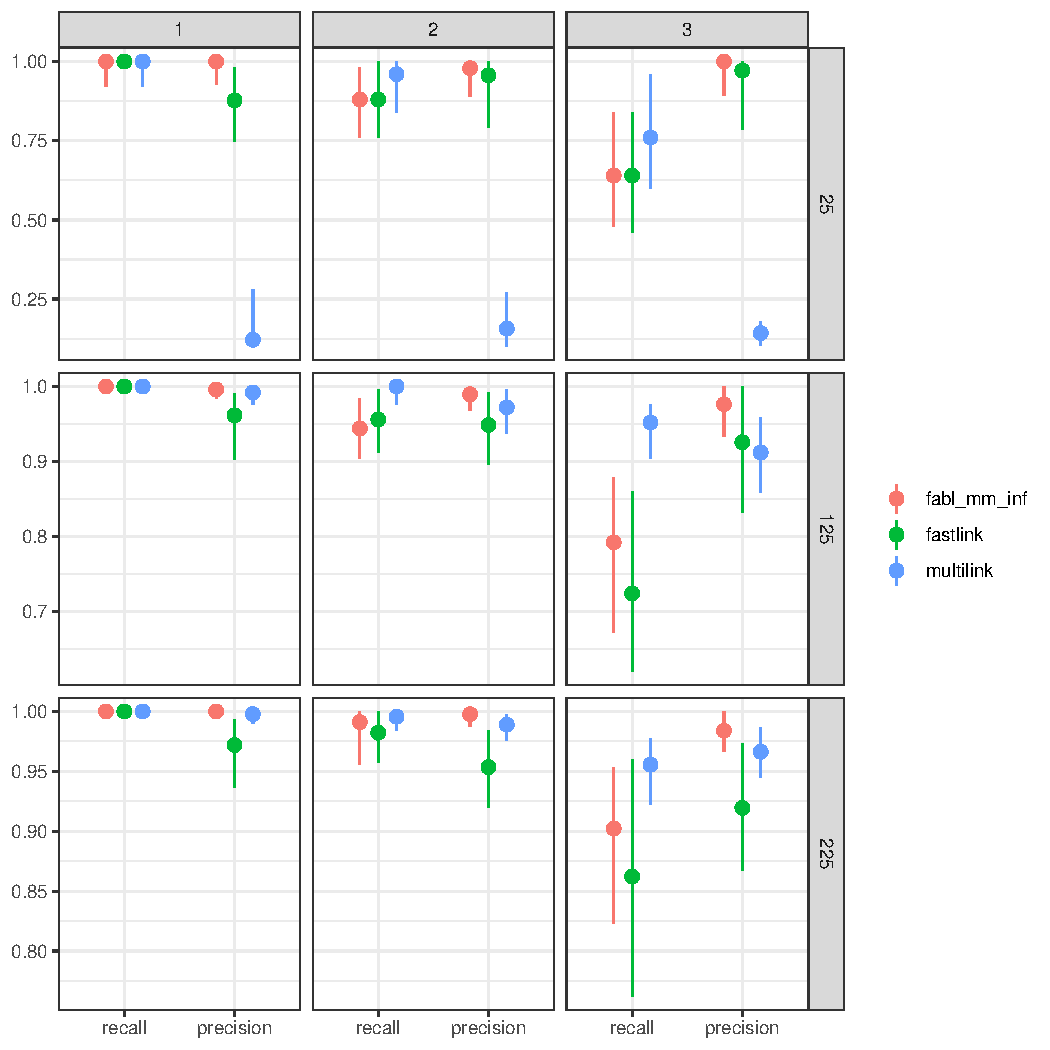
\includegraphics[width=0.8\textwidth]{../Rplots.pdf}
%	\caption{Sadinle Simulation}
%	\label{fig:sadinle}
%\end{figure}
%
%
%NOTE: I've included fastlink (without Jaro) in this image for the time being. However, there is currently no way through fastlink to produce estimates that respect the 2-to-1 matchings while enforcing transitivity. 
%
%\section{Case Study}
%
%In the current analysis of NCVR, I have deduplicated file $B$, and left $A$ with duplicates. I compare five approaches: standard fabl, fabl with multiple match, fabl swap (where I denote $B$ as the file with duplicates and $A$ is duplicate free), fastlink, and fastlink with the Jaro correction. For each method, links are declared with a 0.5 probability cut off, and fabl, fabl\_mm, use the post processing to ensure transitivity. Results are in Table \ref{table:ncvr_results}.
%
%\begin{table}[t]
%		\centering
%\begin{tabular}{l|rrr}
%
%	method & recall & precision & f\_measure\\
%	\hline
%	fabl & 0.9743739 & 0.9798799 & 0.9771191\\
%	\hline
%	fabl\_mm & 0.9891623 & 0.9735309 & 0.9812843\\
%	\hline
%	fabl\_swap & 0.9842840 & 0.9420737 & 0.9627164\\
%	\hline
%	fastlink & 0.9988472 & 0.8494865 & 0.9181321\\
%	\hline
%	fastlink\_jaro & 0.9514490 & 0.9664229 & 0.9588775\\
%\end{tabular}
%\caption{Accuracy results for NCVR}
%\label{table:ncvr_results}
%\end{table}
%
%We see that the multiple match has the highest f-measure. The "fabl swap" method has decently high recall, but precision suffers because there is no post processing step. 


%We conduct linkage when matching records exhibit 1, 2, and 3 errors across the four fields, and when there are 25, 125, and 225 records in $B$ that have matching records in $A$. To test  Under each of these settings, we use 100 pairs of simulated data files in order to obtain uncertainty quantification on our performance metrics.

%The simulations employ a collection of synthetic data files with varying amounts of error and overlap (the number of records in common across files). Following methods proposed by \cite{christen_pudjijono2009} and \cite{christen_vatsalan2013}, clean records are first simulated from frequency tables for first name, last name, age, and occupation in Australia. Fields are then chosen for distortion uniformly at random. Names are subject to string insertions, deletions and substitutions, as well as common keyboard, phonetic, and optical recognition errors. Age and occupation are distorted through keyboard errors and missingness. These synthetic data files are available in the supplement to \cite{sadinle_bayesian_2017}.
%
%We create comparison vectors according to the default settings of the \texttt{compareRecords} function from the \texttt{BRL} package, shown in Table \ref{Tab:sadinle_simulation_cutoffs}. Each simulation identifies matched individuals between two data files, each with 500 records. We conduct linkage when matching records exhibit 1, 2, and 3 errors across the four fields, and when there are 50, 250, and 450 individuals in common across data files. Under each of these settings, we use 100 pairs of simulated data files in order to obtain uncertainty quantification on our performance metrics. We use uniform priors for the $\bm{m}$, $\bm{u}$, and $\pi$ parameters, with $\alpha_{fl} = \beta_{fl} = 1$ for all $f$ and $l$. We run the Gibbs sampler for 1000 iterations, and discard the first 100 as burn-in. We calculate Bayes estimates $\hat{\bm{Z}}$ of the linkage structure using the  loss function and post-processing procedure described in Supplement \ref{bayes-estimate}. Traceplots for parameters of interest for one example simulation are provided in Supplement \ref{app:appendix-sim}; they show no obvious concern over MCMC convergence. We also replicate this simulation allowing \texttt{fabl} to leave some components of the linkage structure undetermined and left for clerical review; those results are in Supplement \ref{partial}.


%Show accuracy under various settings of maximum cluster size for different algorithms. Recall will fall very quickly for \texttt{fabl}. Since we can't use Jaro, precision for \texttt{fastLink} will be poor.  Multilink may be very dependent on correctly specifying $K$. This multiple match approach should remain strong in all settings. 

\bibliographystyle{agsm}
\bibliography{biblio}

\section{Appendix}
\label{sec:appendix}

\subsection{Derivation of Sequential Sampler}\label{app:sequential-sampler}
We now provide the derivation of the sequential sampler, following the argument presented in Section \ref{sec:joint-distribution}. Suppose $B_j$ has been linked to $k$ records in $A$. Let $Z_{j, -k} = (Z_{j, 1}, \ldots, Z_{j, k-1})$ denote the vector of records already linked to $B_j$. When $B_j$ has no additional link in $A$, the contribution to the likelihood is a product of the $u$ parameters for all remaining records. That is, 
\begin{align}
	p(\Gamma_{.j}| \bm{m}, \bm{u}, \pi, Z_{j, k} = \emptyset, Z_{j, -k} = q_{-k}) = \prod_{i \notin Z_{j, -k}} \prod_{f=1}^{F}\prod_{l=1}^{L_f} u_{fl}^{I(\gamma_{ij}^f = l)I_{obs}(\gamma_{ij}^f)} = c_{Z_{j, -k}}.
\end{align}

When $Z_{j, k} = q_k$ for some $q_k > 0$, we have
\begin{align}
	p(\Gamma_{.j}| \bm{m}, \bm{u}, \pi,  Z_{j, k} = q_k, Z_{j, -k} = q_{-k}) &=\prod_{f=1}^{F}\prod_{l=1}^{L_f} m_{fl}^{I(\gamma_{q_k, j}^f = l)I_{obs}(\gamma_{q_k, j}^f)}  \prod_{i \notin (q_{-k}, q_k)}\prod_{f=1}^{F}\prod_{l=1}^{L_f} u_{fl}^{I(\gamma_{ij}^f = l)I_{obs}(\gamma_{ij}^f)} \\
	&=\prod_{f=1}^{F}\prod_{l=1}^{L_f} \left(\frac{m_{fl}}{u_{fl}} \right)^{I(\gamma_{q_k, j}^f = l)I_{obs}(\gamma_{q_k, j}^f)}  \prod_{i \notin (Z_{j, -k}}\prod_{f=1}^{F}\prod_{l=1}^{L_f} u_{fl}^{I(\gamma_{ij}^f = l)I_{obs}(\gamma_{ij}^f)} \\
	&= c_{Z_{j, -k}} w_{q_k, j}
\end{align}
To obtain the posterior, we multiply by the prior in (\ref{eqn:sequential_prior}). The posterior distribution this is given by
\begin{align}\label{eqn:sequential-posterior-full}
	p(Z_{j, k} = q_k|Z_{j, k-1}, \eta_k, \bm{m}, \bm{u}, \gamma) &=
	\frac{\left(\frac{\eta_k}{n_A - (k - 1)}c_{Z_{j, -k}} w_{q_k, j}\right)^{I(q_k \in N_{j, k})} + \left(c_{Z_{j, -k}}(1 - \eta_k)\right)^{I(q_k = \emptyset)}}{\frac{\eta_k}{n_A - (k - 1)}c_{Z_{j, -k}} \sum_{i \notin Z_{j, -k}} w_{ij} + c_{Z_{j, -k}}(1 - \eta_k)} \\
	&=
	\frac{\left(\frac{\eta_k}{n_A - (k - 1)}w_{q_k, j}\right)^{I(q_k \in N_{j, k})} + (1 - \eta_k)^{I(q_k = \emptyset)}}{\frac{\eta_k}{n_A - (k - 1)}\sum_{i \notin Z_{j, -k}} w_{ij} +(1 - \eta_k)} \\
	&\propto \begin{cases}
		\frac{\eta_k}{n_A - (k - 1)} w_{q_k, j}, & q_k \in N_{j, k}, \\
		1 - \eta_k, & q_k= \emptyset.
	\end{cases}
\end{align}


%\subsection{Extended Proof} \label{app:extended-proof}
%\begin{align*}
%	p\left(Z_j  = q |\gamma, \bm{m}, \bm{u}, \pi\right) &\propto \frac{(n_A - |q|)!|q|!}{n_A!} \pi_{|q|} \prod_{i \in q} w_{ij} \\
%	&= \prod_{c = 1}^{|q|} \frac{1}{n_A - (c + 1)} (1 - \eta_{|q|+1}) |q|!\prod_{c = 1}^{|q|} \eta_{|q|} \prod_{c = 1}^{|q|} w_{q_c, j} \\
%	&= (1 - \eta_{|q|+1}) |q|!\prod_{c = 1}^{|q|} \frac{\eta_{|q|} }{n_A - (c + 1)}  \prod_{c = 1}^{|q|} w_{q_c, j} \\
%	&= p(Z_{j, |q|+1} = \emptyset| \eta_{|q|})|q|! \prod_{c = 1}^{|q|} p(Z_{j, c} = q_c|\eta_c) p(\Gamma_{.j}| \bm{m}, \bm{u}, \bm{\eta}, q_c \in Z_j) \\
%	&\propto p(Z_{j, |q|+1} = \emptyset | \Gamma_{.j}, \bm{m}, \bm{u}, \bm{\eta}) |q|!\prod_{c = 1}^{|q|} p(Z_{j, c} = q_c|\Gamma_{.j}, \bm{m}, \bm{u}, \bm{\eta}).
%\end{align*}
%
%\begin{align}
%	p\left(Z_j  = q|\gamma, \bm{m}, \bm{u}, \pi \right) &= \frac{\frac{(n_A - |q|)! |q|!}{n_A!} \pi_{|q|} c_j \prod_{i \in q} w_{ij}}{\sum_{h \in \mathcal{Z}} \frac{(n_A - |h|)! |h|!}{n_A!} \pi_{|h|} c_j \prod_{i \in h} w_{ij}} \\
%	&= \frac{\frac{(n_A - |q|)! |q|!}{n_A!} \pi_{|q|} \prod_{i \in q} w_{ij}}{\sum_{h \in \mathcal{Z}} \frac{(n_A - |h|)! |h|!}{n_A!} \pi_{|h|} \prod_{i \in h} w_{ij}} \\
%	&\propto \frac{(n_A - |q|)! |q|!}{n_A!} \pi_{|q|} \prod_{i \in q} w_{ij}
%\end{align}
%
%\begin{align}
%	\prod_{c = 1}^{|q|} p\left(Z_{j, c} = q_c|\gamma, \bm{m}, \bm{u}, \eta_c, Z_{j, c-1} \right) &=  (1 - \eta_{|q|+1}) |q|!\prod_{c = 1}^{|q|} \frac{\eta_{|q|} }{n_A - (c + 1)}  \prod_{c = 1}^{|q|} w_{q_c, j}
%\end{align}


%\subsection{Equivalence of Samplers}
%\brian{This is just brainstorm}
%Let $\sigma(Z_j)$ denote every possible ordering of the elements of $Z_j$. Because we regard each element $\sigma(Z_j)$ as equal, they must be equally likely. Therefore we have
%\begin{align}
%	p(Z_j = q| \Gamma, m, u, \pi) &= \prod_{q' \in \sigma(q)} \prod_{k=1}^{|q|} p(Z_{j, k} = q'_k| \Gamma, m, u, \eta_k, Z_{j, k-1}) \\
%	&= |q|! \prod_{k=1}^{|q|} p(Z_{j, k} = q_k| \Gamma, m, u, \eta_k, Z_{j, k-1})
%\end{align}
%
%Right after equation 14, I show the that numerators in the two samplers are equal. Does this in a sense imply that their denominators must be equal too?

















%
%
%
%Following the observation of \cite{wortman2019} and elaborated by \cite{kundinger_2023}, when $B_j$ does not link to any record in $A$ (such that $|Z_j| = 0$) the contribution to the likelihood is simply a product of $u$ parameters, which we will call $c_j$:
%\begin{align}
%	p(\Gamma_{.j}| \bm{m}, \bm{u}, \pi, Z_j = \emptyset) = \prod_{i=1}^{n_A}\prod_{f=1}^{F}\prod_{l=1}^{L_f} u_{fl}^{I(\gamma_{ij}^f = l)I_{obs}(\gamma_{ij}^f)} = c_j.
%\end{align}
%When $Z_j = q =  (q_1, \ldots, q_k)$ for some $|q| > 0$, we have
%\begin{align}
%	p(\Gamma_{.j}| \bm{m}, \bm{u}, \pi,  Z_j = q) =\prod_{i \in q}\prod_{f=1}^{F}\prod_{l=1}^{L_f} m_{fl}^{I(\gamma_{ij}^f = l)I_{obs}(\gamma_{ij}^f)}  \prod_{i \notin q}\prod_{f=1}^{F}\prod_{l=1}^{L_f} u_{fl}^{I(\gamma_{ij}^f = l)I_{obs}(\gamma_{ij}^f)}.
%\end{align}
%We multiply and divide by the $u$ parameters for the matching record pairs to obtain
%\begin{align}
%	p(\Gamma_{.j}| \bm{m}, \bm{u}, \pi, Z_j = q) &= \prod_{i \in q}\prod_{f=1}^{F}\prod_{l=1}^{L_f} \left(\frac{m_{fl}}{u_{fl}}\right)^{I(\gamma_{ij}^f = l)I_{obs}(\gamma_{ij}^f)}  \prod_{i = 1}^{n_A}\prod_{f=1}^{F}\prod_{l=1}^{L_f} u_{fl}^{I(\gamma_{ij}^f = l)I_{obs}(\gamma_{ij}^f)} \\
%	&= c_j \prod_{i \in q} w_{ij} .
%\end{align}
%
%Lastly, we multiply the likelihood by the prior in (\label{eqn:z}) to obtain the posterior distribution. Since $Z_j$ is a categorical random variable with every possible combination of the records in $A$ as its potential values, its distribution is given by the likelihood of one outcome divided by the sum of the likelihood for all outcomes. For $Z_j = q$ where $|q| = k$, we have
%\begin{align}\label{eqn:joint_posterior}
%	p\left(Z_j  = q|\gamma, \bm{m}, \bm{u}, \pi \right) &= \frac{\frac{(n_A - k)! k!}{n_A!} \pi_{k} c_j \prod_{i \in q} w_{ij}}{\sum_{h \in \mathcal{Z}} \frac{(n_A - |h|)! |h|!}{n_A!} \pi_{|h|} c_j \prod_{i \in h} w_{ij}} \\
%	&= \frac{\frac{(n_A - k)! k!}{n_A!} \pi_{k} \prod_{i \in q} w_{ij}}{\sum_{h \in \mathcal{Z}} \frac{(n_A - |h|)! |h|!}{n_A!} \pi_{|h|} \prod_{i \in h} w_{ij}} \\
%	&\propto \frac{(n_A - k)! k!}{n_A!} \pi_{k} \prod_{i \in q} w_{ij}
%\end{align}
%Importantly, the constant $c_j$ is not found in the final expression because the probability mass associated with every potential value for $Z_j$ shares the same $c_j$. This does not occur due to proportionality. 

\end{document}
